\section{Implementation}
We have implemented the lens synthesis algorithm in $n$ lines of OCaml code.

\subsection{Synthesis Overview}
\begin{figure}
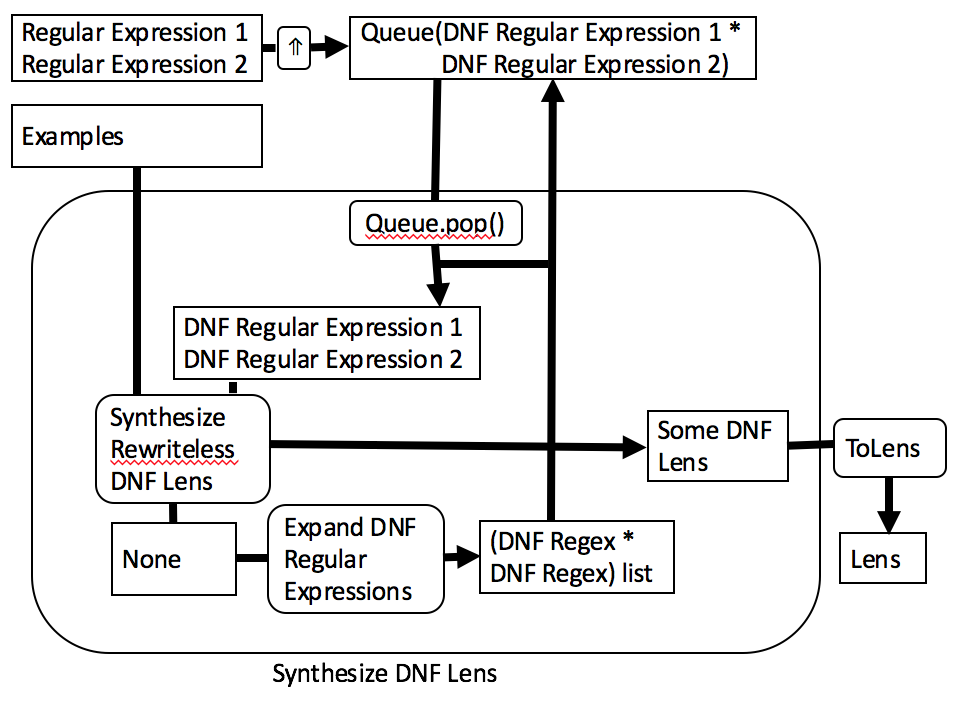
\includegraphics[scale=.5]{synth-lens-schematic.png}
\label{fig:synth-lens-schematic}
\end{figure}
The synthesis algorithm is shown in a schematic diagram in 
Figure~\ref{fig:synth-lens-schematic}.  The algorithm takes in a pair of
regular expressions, and examples, and converts the regular expressions into
DNF regular expressions, using \ToDNFRegex{}.
These then get enqueued, and SynthDNFLens, where the bulk of the work
occurs.

In SynthDNFLens, the highest priority DNF regular expression pair is popped.
Then, SynthRewritelessDNF sees if a DNF lens which satisfies the examples, which
does not include any applications of the rewrite rule, can be found.
If none are found, then each rewrite is applied once on each side of the regular
expressions.
This new list of DNF regular expression doubles is enqueued, and SynthDNFLens is
called again.
If one is found, this DNF lens gets converted to a normal lens, and is returned
to the user.

\subsection{Priority Queue}
The priority queue is implemented with a list implementation of a priority queue.
We say that the lower the priority value, the higher the priority.
The priority value of an element is based on the number of expansions that have been
preformed, combined with the distance between the two regular expressions, based
on a psuedometric $\Distance$ we have implemented.  This pseudometric is implemented
as the sum of simpler pseudometrics,
$\Distance = \Distance_{size}+\Distance_{dist}$.

$\Distance_{size}$ is defined as merely the difference in the sizes of the DNF
regular expressions.
$\Distance_{size}(\DNFRegex,\DNFRegexAlt)=\AbsOf{\Size(\DNFRegex)-\Size(\DNFRegexAlt)}$

$\Distance_{dist}$ captures how far apart the distribution of
user defined regular expressions are.
The distribution of user defined regular expressions can be viewed as an
infinite dimensional free module over the integers, \Module{}.
The basis for this is $\SetOf{1*(\RegexVariable,n) | n\in\Nats, \RegexVariable
\text{ is a user defined regular expression}}$
DNF regular expressions with variables can map into this with a function by
counting the number of user defined data types present at a given level.
The formal definition for this mapping is given by the function \GetDist{}.

\begin{definition}\leavevmode\\
\label{def:getdist}
\begin{tabular}{@{}L@{}L@{}}
\GetDist(\DNFOf{\Sequence_1;\ldots;\Sequence_n}) &
=\GetDist(\Sequence_1)+\ldots+\GetDist(\Sequence_n)\\
\GetDist(\SequenceOf{\String_0;\Atom_1;\ldots;\Atom_n;\String_n}) &
=\GetDist(\Atom_1)+\ldots+\GetDist(\Atom_n)\\
\GetDist(\RegexVariable)&=1*(\RegexVariable,1)\\
\GetDist(\IterateLens{\DNFLens})&=\phi(\GetDist(\DNFLens))
\end{tabular}

where $\phi$ is the linear map sending $1*(\RegexVariable,n)$ to
$1*(\RegexVariable,n+1)$
\end{definition}

Using this, we now have a mapping from regular expressions into the distribution
of user defined regular exprssions.

$\Distance_{dist}(\DNFRegex,\DNFRegexAlt)=\LOneNorm(\phi(\DNFRegex),\phi(\DNFRegexAlt))$
where \LOneNorm{} is the taxicab metric on \Module{}.
The priority of a pair of DNF regular expressions, $(\DNFRegex{},\DNFRegexAlt{})$,
is $\Distance(\DNFRegex{},\DNFRegexAlt{})+8*expansion_count$.
Keeping track of expansion count is important as it allows for lower priority
expansions to be eventually popped, instead of getting stuck doing incorrect,
increasingly deep expansions whose DNF regular expressions have a low distance.
\afm{should i do an example, or is that going into too much detail?}
Experimentally, 8 was a good value for how much weight the expansion
count should get in the priority.  It allows for not getting stuck in a local
minima in the search space, while still allowing for the distance to choose the
correct expansion the majority of the time.

\subsection{SynthRWLessDNF}
We find an efficient way to synthesize DNF lenses which do not use rewrites.
